\documentclass{report}
\usepackage[utf8]{inputenc}
\usepackage{amsmath}
\usepackage{graphicx}

\title{Eksamensnoter - Divide and Conquer}
\author{André Oskar Andersen (wpr684)}
\date{\today}

\begin{document}
\maketitle

\section*{2.3 Designing algorithms}
\subsection*{2.3.1 The divide-and-conquer approach}
\begin{itemize}
    \item The divide-and-conquer paradigm involves three steps at each level of the recursion:
    \begin{itemize}
        \item \textbf{Divide} the problem into a number of subproblems that are smaller instances of the same problem
        \item \textbf{Conquer} the subproblems by solving them recursively. If the subproblem sizes are small enough, however, just solve the subroblems in a straightforward manner
        \item \textbf{Combine} the solutions to the subproblems into the solution for the original problem
    \end{itemize}
    \item The \textit{merge sort} algorithm closely follows the divide-and-conquer paradigm:
    \begin{itemize}
        \item \textbf{Divide:} Divide the \textit{n}-element sequence to be sorted into two subsequences of $n/2$ elements each
        \item \textbf{Conquer:} Sort the two subsequences recursively using merge sort
        \item \textbf{Combine:} Merge the two sorted subsequences to produce the sorted answer
    \end{itemize}
\end{itemize}
\subsection*{2.3.2 Analyzing divide-and-conquer algorithms}
\begin{itemize}
    \item When an algorithm contains a recursive call to itself, we can often describe its running time by a \textit{recurrence equation} or \textit{recurrence}, which describes the overall running time on a problem of size \textit{n} in terms of the running time on smaller inputs. When can then use mathematical tools to solve the recurrence and provide bounds on the performance of the algorithm
    \item We let $T(n)$ be the running time on a problem of size \textit{n}. If the problem size is small enough, say $n \leq c$ for some constant \textit{c}, the straightforward solution takes $\Theta(1)$. Suppose that our division of the problem yields \textit{a} subproblems, each of which is $1/b$ tbe size of the original. It takes time $T(n/b)$ to solve one subproblem of size $n/b$, and so it takes time $aT(n/b)$ to solve \textit{a} of them. If we take $D(n)$ time to divide the problem into subproblems and $C(n)$ time to combine the solutions to the subproblems into the solution to the original problem, we get the recurrence
    \[
        T(n) = 
        \begin{cases}
            \Theta(1) & \textit{i$n\leq c$} \\
            aT(n/b) + D(n) + C(n) & \text{otherwise}
        \end{cases}    
    \]
\end{itemize}
\subsubsection*{Analysis of merge sort}
\begin{itemize}
    \item We reason as follows to set up the recurrence for $T(n)$, the worst-case running time of merge sort on \textit{n} numbers. Merge sort on just one element takes constant time. When we have $n > 1$ elements ,we break down the running time as follows:
    \begin{itemize}
        \item \textbf{Divide:} The divide step just computes the middle of the subarray, which takes constant time. Thus, $D(n) = \Theta(1)$
        \item \textbf{Conquer:} We recursively solve two subproblems, each of size $n/2$, which contributes $2T(n/2)$ to the running time
        \item \textbf{Combine:} Merging \textit{n}-elements takes $\Theta(n)$, and so $C(n) = \Theta(n)$
    \end{itemize}
    \item Letting $D(n) + C(n) = \Theta(1) + \Theta(n) = \Theta(n)$ and adding this to the $2T(n/2)$ term from the "conquer" step gives the recurrence for the worst-case running time $T(n)$ of merge sort:
    \[
        T(n) = 
        \begin{cases}
            \Theta(1) & \text{if $n = 1$} \\
            2T(n/2) + \Theta(n) & \text{if $n > 1$}
        \end{cases}    
    \]
    \item We can use an \textit{recursion tree} to understand why $T(n) = \Theta(n \lg n)$. This is done, by first rewritting $T(n)$:
    \[
        T(n) = 
        \begin{cases}
            c & \text{if $n = 1$} \\
            2T(n/2) + cn & \text{if $n > 1$}
        \end{cases}    
    \]
    where \textit{c} represents the time requiered to solve problems of size 1 as well as the time per array element of the divide and combine steps (it is unlikely that the same constant represents both. We can get around this by letting \textit{c} be the larger/lesser of these times and understanding that our recurrence gives an upper/lower bound on the running time).
    \begin{center}
        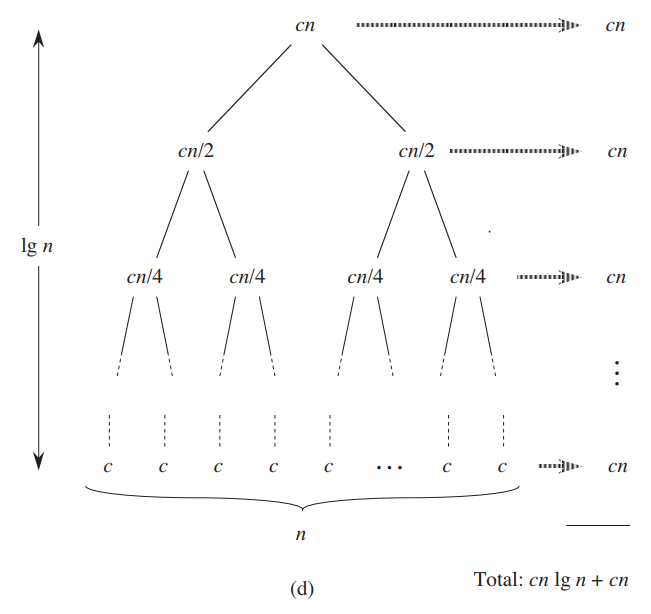
\includegraphics[width = 10 cm]{../entities/merge_sort_recursion_tree.png}
    \end{center}
    Next, we add the costs across each level of the tree. In general, the level \textit{i} below the top has $2^i$ nodes, each contributing a cost of $c(n/2^i)$, so that the \textit{i}th level below the top has total cost $2^ic(n/2^i) = cn$. \\
    The toal number of levels of the recursion tree is $\lg n + 1$, where \textit{n} is the number of leaves, corresponding to the input size. An informal inductive argument justifies this claim:
    \begin{itemize}
        \item The base case occurs when $n = 1$, in which case the tree has only one level. Since $\lg 1 = 0$, we have that $\lg n + 1$ gives the correct number of levels.
        \item Assume, that the number of levels of a recursion tree with $2^i$ leaves is $\lg 2^i + 1 = i + 1$. Because we are assuming that the input size is a power of 2, the next input size to consider is $2^{i + 1}$. A tree with $n = 2^{i + 1}$ leaves has one more level than a tree with $2^i$ leaves, and so the total number of levels is $(i + 1) + 1 = \lg 2^{i + 1} + 1$.
    \end{itemize}
    To compute the total cost represented by the recurrence $T(n)$, we add up the costs of all the levels; the tree has $\lg n + 1$ levels, each costing $cn$, for a total of $cn(\lg n + 1) = cn \lg n + cn = \Theta(n \lg n)$.
\end{itemize}

\section*{4 Divide-and-Conquer}
\begin{itemize}
    \item When the subproblems are large enough to solve recursively, we call that the \textit{recursive case}. Once the subproblems become small enough that we no longer recurse, we say that the recursion "bottoms, out" and that we have gotten down to the \textit{base case}.
\end{itemize}
\textbf{Recurrences}
\begin{itemize}
    \item Recurrences go hand in hand with the divide-and-conquer paradigm, because they give us a natural way to characterize the running time of divide-and-conquer algorithms
    \item There are three methods for solving recurrences - that is, for obtaining asymptotic "$\Theta$" or "$O$" bounds on the solution:
    \begin{itemize}
        \item In the \textit{substitution method}, we guess a bound and then use mathematical induction to prove our guess correct
        \item The \textit{recursion-tree method} converts the recurrence into a tree whose nodes represent the costs incurred at various levels of the recursion. We use techniques for bounding summations to solve the recurrence.
        \item The \textit{master method} provides bounds for recurrences of the form $T(n) = aT(n/b) + f(n)$, where $a \geq 1, b > 1$, and $f(n)$ is a given function. A recurrence of this form characterizes a divide-and-conquer algorithm that creates \textit{a} subproblems, each of which is $1/b$ the size of the original problem, and in which the divide and combine steps together take $f(n)$ time.
    \end{itemize}
\end{itemize}
\textbf{Technicalities in recurrences}
\begin{itemize}
    \item In practice, we neglect certain technical details when we state and solve recurrences.
    \item Boundary conditions represent a class of details that we typically ignore. Since the ruuning time of an algorithm on a constant-sized input is a aconstant, the recurrences that arise from the running times of algorithms generally have $T(n) = \Theta(1)$ for sufficiently small \textit{n}. For convenience, we shall generally omit statements of the boundary conditions of recurrences and assume that $T(n)$ is constant for small \textit{n}. For example, we normally state the recurrence
    \[
        T(n) = 
        \begin{cases}
            \Theta(1) & \text{if $n = 1$} \\
            2T(n/2) + \Theta(n) & \text{if $n >1$}
        \end{cases}    
    \]
    as
    $$T(n) = 2T(n/2) + \Theta(n)$$
    without explicitly giving values for small \textit{n}.l The reason is that alothough changing the values of $T(1)$ changes the exact solution to the recurrence, the solution typically doesn't change by more than a constant factor, and so the order of growth is unchanged.
    \item Floors and ceilings are another class of details that we typically ignore. For example, if we call merge-sort on \textit{n} elements when \textit{n} is odd, we end up with subproblems of size $\left \lfloor{n/2} \right \rfloor \textit{ and } \left \lceil{n/2} \right \rceil$. Neither size is actually $n/2$, because $n/2$ is not an integer when \textit{n} is odd.
\end{itemize}
\subsection*{4.3 The substitution method for solving recurrences}
\begin{itemize}
    \item The \textit{substitution method} for solving recurrences comprises two steps:
    \begin{enumerate}
        \item Guess the form of the solution
        \item Use mathematical induction to find the constants and show that the solution works
    \end{enumerate}
    \item We substitute the guessed solution for the function when applying the inductive hypothesis to smaller values; hence thename "substitution method".
    \item We can use the substitution method to establish either upper or lower bounds on a recurrence. As an example, let us determine an upper bound on the recurrence
    $$T(n) = 2T(\left \lfloor{n/2} \right \rfloor) + n$$
    We guess that the solution is $T(n) = O(n \lg n)$. The substitution method requires us to prove that $T(n) \leq cn \lg n$ for an appropriate choice of the constant $c > 0$. We start by assuming that his bound holds for all positive $m < n$, in particular $m = \left \lfloor{n/2} \right \rfloor$, yielding $T(\left \lfloor{n/2} \right \rfloor) \leq c \left \lfloor{n/2} \right \rfloor \lg(\left \lfloor{n/2} \right \rfloor)$. Subtituting into the recurrence yields
    $$T(n) = 2T(\left \lfloor{n/2} \right \rfloor) + n$$
    $$\leq 2(c \left \lfloor{n/2} \right \rfloor \lg(\left \lfloor{n/2} \right \rfloor)) + n$$
    $$\leq cn \lg(n/2) + n$$
    $$= cn \lg n - cn \lg 2 + n$$
    $$= cn \lg n - cn + n$$
    $$\leq cn \lg n$$
    where the last step holds as long as $c \geq 1$.
    \item Mathematical induction now requires us to show that our solution holds for the boundary conditions. Typically, we do so by showing that the boundary conditions are suitable as base cases for the inductive proof. For this example, we must show that we an choose the constant \textit{c} large enough so that the bound $T(n) \leq cn \lg n$ works for the boundary conditions as well. This requirement can sometimes lead to problems:
    \begin{enumerate}
        \item Let us assume, that $T(1) = 1$ . Then for $n = 1$, the bound $T(n) \leq cn \lg n$ yields $T(1) \leq c1 \lg 1 = 0$, which is at odds with $T(1) = 1$
    \end{enumerate}
    We can overcome this obstacle:
    \begin{enumerate}
        \item By observing that for $n > 3$, the recurrence does not depend directly on $T(1)$, we can replace $T(1)$ by $T(2)$ and $T(3)$ as the base cases in the inductive prrof, letting $n_0 = 2$.
        \item We derive from the recurrence that $T(2) = 4$ and $T(3) = 5$.
        \item Now we can complete the inductive proof that $T(n) \leq cn \lg n$ for some constant $c \geq 1$ by choosing \textit{c} large enough so that $T(2) \leq c2 \lg 2$ and $T(3) \leq c3 \lg 3$. As it turns out, any choice of $c \geq 2$ suffices for the base cases of $n = 2$ and $n = 3$ to hold.
    \end{enumerate}
\end{itemize}
\textbf{Subtleties}
\begin{itemize}
    \item Consider the recurrence
    $$T(n) = T(\left \lfloor{n/2} \right \rfloor) + \left \lceil{n/2} \right \rceil + 1$$
    We guess that the solution is $T(n) = O(n)$, and we try to show that $T(n) \leq cn$ for an appropriate choice of the constant \textit{c}. Substituting our guess in the recurrence, we obtain
    $$T(n) \leq c \left \lfloor{n/2} \right \rfloor + c \left \lceil{n/2} \right \rceil + 1 = cn + 1$$
    which does not impoy $T(n) \leq cn$ for any choice of \textit{c}; we are off only by the constant 1. We overcome our difficulty by subtracting a lower-order term from our previous guess. Our new guess it $T(n) \leq cn - d$, where $d \geq 0$ is a constant. We now have
    $$T(n) \leq (c \left \lfloor{n/2} \right \rfloor - d) + (c \left \lceil{n/2} \right \rceil) + 1 = cn - 2d + 1 \leq cn - d$$
    as long as $d \geq 1$
\end{itemize}
\subsection*{4.4 The recursion-tree method for solving recurrences}
\begin{itemize}
    \item Drawing out a recursion tree serves as a traghtforward way to devise a good guess, which then can be verified using the \textit{substitution method}. If you are very careful when drawing out a recursion tree and summing the costs, however. you can use a recursion tree as adirect proof of a solution to a recurrence.
    \item When using a recursion tree to generate a good guess, you can often tolerate a small amount of "sloppiness", since you will be verifying your guess later. 
    \item In a \textit{recursion tree}, each node represents the cost of a single subproblem somewhere in the set of recursive function invocations. We sum the costs within each level of the tree to obtain a set of per-level costs, and then we sum all the per-level costs to determine the total cost of all levels of the recursion
    \item An example on how to come up with a good guess using an recursion tree, can be seen in section 2.3.2 where merge sort is analysed.
\end{itemize}
\subsection*{4.5 The master method for solving recurrences}
\begin{itemize}
    \item The master method provides a "cookbook" method for solving recurrences of the form
    $$T(n) = aT(n/b) + f(n)$$
    where $a \geq 1$ and $b > 1$ are constants and $f(n)$ is an asymptotically positive function.
    \item The recurrence describes the running time of an algorithm that divides a problem of size \textit{n} into \textit{a} subproblems, each of size $n/b$, where \textit{a} and \textit{b} are positive constants. The \textit{a} subproblems are solvd recursively, each in time $T(n/b)$. The function $f(n)$ encompasses the cost of dividing the problem and combining the results of the subproblems.
\end{itemize}
\textbf{The master theorem}
\begin{itemize}
    \item The master method depends on the following theorem:
    \begin{itemize}
        \item Let $a \geq 1$ and $b > 1$ be constants, let $f(n)$ be an asymptotically positive function, and let $T(n)$ be defined on the nonnegative integers by the recurrence $T(n) = aT(n/b) + f(n)$ where we interpret $n/b$ to mean either $\left \lfloor{n/2} \right \rfloor$ or $\left \lceil{n/2} \right \rceil$. Then $T(n)$ has the following asymptotic bounds:
        \begin{enumerate}
            \item If $f(n) = O(n^{\log_b a -\epsilon})$ for some constants $\epsilon > 0$, then $T(n) = \Theta(n^{\log_b a})$
            \item If $f(n) = \Theta(n^{\log_b a})$, then $T(n) = \Theta(n^{\log_b a} \lg n)$
            \item If $f(n) = \Omega(n^{\log_b a + \epsilon})$ for some constant $\epsilon > 0$, and if $af(n/b) \leq cf(n)$ for some constant $c < 1$ and all sufficiently large \textit{n}, then $T(n) = \Theta(f(n))$
        \end{enumerate}
    \end{itemize}
\end{itemize}
\textbf{Using the master method}
\begin{itemize}
    \item Consider
    $$T(n) = 9T(n/3) + n$$
    For this recurrence, we have $a = 9$, $b = 3$, $f(n) = n$, and thus we have that $n^{\log_b a} = n^{\log_3 9} = \Theta(n^2)$. Since $f(n) = O(n^{\log_3 0 - \epsilon})$, where $\epsilon = 1$, we can apply case 1 and conclude that the solution is $T(n) = \Theta(n^2)$
\end{itemize}
\section*{8 Sorting in Linear Time}
\begin{center}
    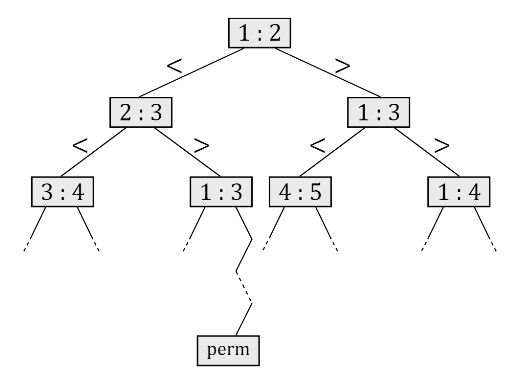
\includegraphics[width = 10 cm]{../entities/decision_tree_lower_bound_comparison_sort.png}
\end{center}
\subsection*{8.1 Lower bounds for sorting}
\begin{itemize}
    \item In a comparison sort, we use only comparisons between elements to gain order information about an input sequence $\{a_1, a_2, ..., a_n\}$. That is, given two elements $a_i$ and $a_j$, we perform one of the tests $a_i < a_j, a_i \leq a_j, a_i = a_j, a_i > a_j, a_i \geq a_j$ to determine their relative order. We maynot inspect the values of the elements or gain order information about them in any other way
    \item We assume without loss of generality, that all the input elements are distinct. Thus, $a_i = a_j$ are useles, so we can assume that no comparisons of this form are made. We also note that the other comparisons are all equivalent in that they yield identical information. We therefore assume that all comparisons have the form $a_i \leq a_j$
\end{itemize}
\textbf{The decision-tree model}
\begin{itemize}
    \item We can view comparison sorts abstractly in terms of decision trees, by annotating each internal node by $i:j$ for some \textit{i} and \textit{j} in the range $1 \leq i; j \leq n$, where \textit{n} is the number of elements in the input sequence. We also annotate each leaf by a permutation $\{\pi(1), \pi(2), ..., \pi(n)\}$. The execution of the sorting algorithm corresponds to tracing a simple path from the root of the decision tree down to a leaf. Each internal node indicates a comparison $a_i \leq a_j$. The left subtree then dictates subsequent comparisons once we know that $a_i \leq a_j$, and the right subtree dictates subsequent comparisons knowing that $a_i > a_j$.
\end{itemize}
\textbf{A lower bound for the worst case}
\begin{itemize}
    \item The length of the longest simple path from the root of a decision tree to any of its reachable leaves represents the worst-case number of comparisons that the corresponding sorting algorithm performs. Consequently, the worst-case number of comparisons for a given comparison sort algorithm equals the height of its decision tree. A lower bound on the heights of all decision trees i which each permutation appears as a reachable leaf is therefore a lower bound on the running time of any comparison sort algorithm.
\end{itemize}

\textbf{Theorem 8.1}
\begin{itemize}
    \item Any comparison sort algorithm requires $\Omega(n \lg n)$ comparisons in the worst case \\
    \textbf{proof}:
    \begin{itemize}
        \item Consider a decision tree of height \textit{h} with \textit{l} reachable leaves corresponding to a comparison sort on \textit{n} elements. Because each of the $n!$ permutations of the input appears as some leaf, we have $n! \leq l$. Since a binary tree of height \textit{h} has no more than $2^h$ leaves, we have
        $$n! \leq l \leq 2^h$$
        which, by taking logarithms, implies
        $$h \geq \lg(n!) = \Omega(n \lg n)$$
    \end{itemize}
    \item Since the $O(n \lg n)$ upper bounds on the running times for heapsort and merge sort match the $\Omega(n \lg n)$ worst-case lower bound, heapsort and merge sort are asymptotically optimal comparison sorts.
\end{itemize}

\section*{33 Computational Geometry}
\subsection*{33.4 Finding the closest pair of points}
\begin{itemize}
    \item Consider the problem of finding the closest pair of points in a set \textit{Q} of $n \geq 2$ points.
    \item The divide-and-conquer algorithm for this problem, has a running time described by $T(n) = 2T(n/2) + O(n)$
\end{itemize}
\textbf{The divide-and-conquer algorithm}
\begin{center}
    \includegraphics[width = 10 cm]{../entities/figure_33_11.png}
\end{center}
\begin{itemize}
    \item Each recursive invocation of the algorithm takes as input a subset $P \subseteq Q$ and arrrays $X$ and $Y$, each of which contains all the points of the inpput subset \textit{P}. The points in array \textit{X} are sorted so that their \textit{x}-coordinates are monotonically increasing. Similarly, array \textit{Y} is sorted by monotonically increasing \textit{y}-coordinate.
    \item A given recursive invocation with inputs $P$, $X$, and $Y$ first checks whether $|P| \leq 3$. If so, the invocation simply performs the brute-force method: try all $|P| \choose 2$ pairs of points and return the closest pair. If $|P| > 3$, the recursive invocation carries out the divide-and-conquer paradigm as follows:
    \begin{itemize}
        \item \textbf{Divide}: Find a line \textit{l} that bisects the point set \textit{P} into two equally sized sets $P_L$ and $P_R$. Divide the array \textit{X} into arrays $X_L$ and $X_R$, which contain the points of $P_L$ and $P_R$ respectively, sorted by monotonically increasing \textit{x}-coordinate. Similarly, divide the array \textit{Y} into arrays $Y_L$ and $Y_R$, which contain the points of $P_L$ and $P_R$ respectively, sorted by monotonically increasing \textit{y}-coordinate.
        \item \textbf{Conquer}: Having divided \textit{P} into $P_L$ and $P_R$, make two recursive calls, one to find the closest pair of poitns in $P_L$ and the other to find the closest pair of points in $P_R$. The input to the first call are the subset $P_L$ and arrays $X_L$ and $Y_L$; the second call receives the inputs $P_R$, $X_R$ and $Y_R$. Let the closest-pair distances returned for $P_L$ and $P_R$ be $\delta_L$ and $\delta_R$, respectively, and let $\delta = \min(\delta_L, \delta_R)$
        \item \textbf{Combine}: The closest pair is either the pair with distance $\delta$ found by one of the recursive calls, or it is a pair of points with one point in $P_L$ and the other in $P_R$. If a pair of points has distance less than $\delta$, both points of the pair must be within $\delta$ units of line \textit{l}. Thus, they both must reside in the $2\delta$-wide vertical strip centered at line \textit{l}. To find such a pair, we do the following:
        \begin{enumerate}
            \item Create an array $Y'$, which is the array \textit{Y} with all points not in the $2\delta$-wide vertical strip removed. The array $Y'$ is sorted by \textit{y}-coordinate, just as \textit{Y} is.
            \item For each point \textit{p} in the array \textit{Y'}, try to find points in \textit{Y'} that are within $\delta$ units of \textit{p}. Only the 7 points in \textit{Y'} that follow \textit{p} need to be considered. Compute the distance from \textit{p} to each of these 7 points, and keep track of the closest-pair distance $\delta'$ found over all pairs of points in $Y'$
            \item If $\delta' < \delta$, then the verical strip does indeed contain a closer pair than the recursive calls found. Return this pair and its distance $\delta'$. Otherwise, return the closest pair and its distance $\delta$ found by the recursive calls.
        \end{enumerate} 
    \end{itemize}
\end{itemize}
\textbf{Correctness}
\begin{itemize}
    \item By bottoming out the recursion when $|P| \leq 3$, we ensure that we never try to solve a subproblem consisting of only one point. 
    \item We need only to check the 7 points following each point \textit{p} in array \textit{Y'}; suppose that at some level of the recursion, the closest pair of points is $p_L \in P_L$ and $p_R \in P_R$. Thus, the distance $\delta'$ between $p_L$ and $p_R$ is strictly less than $\delta$. Point $p_L$ must be on or to the left of line \textit{l} and less than $\delta$ units away. Similarly, $p_R$ is on or to the right of \textit{l} and less than $\delta$ units away. Moreover, $p_L$ and $p_R$ are within $\delta$ units of each other vertically. Thus, $p_L$ and $p_R$ are within a $\delta \times 2\delta$ rectangle centered at \textit{l}.
    \item We next show that at most 8 points of \textit{P} can reside within this $\delta \times 2\delta$ rectangle. Consider the $\delta \times \delta$ square forming the left half of this rectangle. Since all points within $P_L$ are at least $\delta$ units apart, at most 4 points can reside within this square. Similarly, at most 4 points in $P_R$ can reside within the $\delta \time \delta$ square forming the right half of the rectangle. Thus, at most 8 points of \textit{P} can reside within $\delta \times 2 \delta$ rectangle.
    \item Now, we can see why we need to check only the 7 points following each point in the array \textit{Y'}. Still assuming that the closest pair is $p_L$ and $p_R$, let us assume that $p_L$ precedes $p_R$ in array \textit{Y'}. Then, $p_R$ is in one of the 7 positions following $p_L$. Thus, we have shown the correctness of the closest-pair algorithm.
\end{itemize}
\end{document}